\documentclass[aspectratio=169]{beamer}
\usetheme{Boadilla}

\usepackage{hyperref}
\usepackage{graphicx}
\usepackage{subcaption}
\usepackage{standalone}
\usepackage[ngerman]{babel}
\usepackage{tikz}
\usepackage{listings}

\title[QDMR]{QDMR ein universeller Code-Plug Editor (CPS) für Linux \& Mac\\ (und vielleicht Windows)}
\subtitle{}

\author{Hannes, DM3MAT}
\institute{\texttt{dm3mat [at] darc [dot] de}}
\date{25. März 2021}

\lstset{ %
basicstyle=\tiny    % the size of the fonts that are used for the line-numbers
}


\newcommand{\repeater}[3]{%
 \node ({#1}) at ({#2}) {%
  \begin{tikzpicture}%
   \draw [black,thick] (-.25,0) -- (0,0.5) -- (0.25,0) -- (-0.25,0);%
   \draw [black,thick,domain=-45:225] plot ({0.2*cos(\x)}, {0.5+0.2*sin(\x)});%
   \draw [black,thick,domain=-45:225] plot ({0.4*cos(\x)}, {0.5+0.4*sin(\x)});%
   \node (xxx) at (0,-.2) {{#3}};%
  \end{tikzpicture}%
 } %
}

\newcommand{\activerepeater}[3]{%
 \node ({#1}) at ({#2}) {%
  \begin{tikzpicture}%
   \draw [black,thick] (-.25,0) -- (0,0.5) -- (0.25,0) -- (-0.25,0);%
   \draw [red,thick,domain=-45:225] plot ({0.2*cos(\x)}, {0.5+0.2*sin(\x)});%
   \draw [red,thick,domain=-45:225] plot ({0.4*cos(\x)}, {0.5+0.4*sin(\x)});%
   \node (xxx) at (0,-.2) {{#3}};%
  \end{tikzpicture}%
 } %
}


\newcommand{\user}[3]{%
 \node ({#1}) at ({#2}) {%
  \begin{tikzpicture}%
   \draw [black,fill=black] (-.25,0) -- (0,0.5) -- (0.25,0) -- (-0.25,0);%
   \draw [black,fill=black] (0,.5) circle (.2); %
   \node (xxx) [text width=0.6cm, align=center] at (-.35cm,-.4) {{#3}};%
  \end{tikzpicture}%
 } %
}

\newcommand{\activeuser}[3]{%
 \node ({#1}) at ({#2}) {%
  \begin{tikzpicture}%
   \draw [red,fill=red] (-.25,0) -- (0,0.5) -- (0.25,0) -- (-0.25,0);%
   \draw [red,fill=red] (0,.5) circle (.2); %
   \node (xxx) [text width=0.6cm, align=center] at (-.35cm,-.4) {{#3}};%
  \end{tikzpicture}%
 } %
}


\begin{document}
\begin{frame}
 \titlepage
\end{frame}

\begin{frame} \frametitle{Übersicht}
 \tableofcontents
\end{frame}


\section{Ganz kurze Einführung in DMR}
\begin{frame} \frametitle{Einführung -- DMR ein Mobilfunknetz für den Amateurfunk} 
\begin{block}{Was ist DMR?}
 \begin{itemize}
  \item Ein digitaler Daten und Sprachübertragungsmodi für UKW.
  \item Gedacht als Ersatz für den analogen Bündelfunk.
  \item Endpunkte werde über \emph{Telefonnummern} identifiziert.
  \item Verwendet 12.5kHz Raster (wie NBFM). 
  \item Erlaubt vernetzten Repeater betrieb (über sog. Sprechgruppen).
  \item Erlaubt durch Kompression das \emph{Bedienen} zweier Endgeräte auf einem physischen Kanal (zwei unabhängige \emph{Zeitschlitze}).
 \end{itemize}
\end{block}
\end{frame}

\begin{frame} \frametitle{Repeaterbetrieb und Direktrufe}
 \begin{block}{Merke}
  Alle DMR Repeater sind untereinander vernetzt und vermitteln Gespräche.
 \end{block}
 \begin{center}
   \documentclass{standalone}
\usepackage{tikz}
\usetikzlibrary{shapes.geometric}
\newcommand{\repeater}[3]{%
 \node ({#1}) at ({#2}) {%
  \begin{tikzpicture}%
   \draw [black,thick] (-.25,0) -- (0,0.5) -- (0.25,0) -- (-0.25,0);%
   \draw [black,thick,domain=-45:225] plot ({0.2*cos(\x)}, {0.5+0.2*sin(\x)});%
   \draw [black,thick,domain=-45:225] plot ({0.4*cos(\x)}, {0.5+0.4*sin(\x)});%
   \node (xxx) at (0,-.2) {{#3}};%
  \end{tikzpicture}%
 } %
}

\newcommand{\activerepeater}[3]{%
 \node ({#1}) at ({#2}) {%
  \begin{tikzpicture}%
   \draw [black,thick] (-.25,0) -- (0,0.5) -- (0.25,0) -- (-0.25,0);%
   \draw [red,thick,domain=-45:225] plot ({0.2*cos(\x)}, {0.5+0.2*sin(\x)});%
   \draw [red,thick,domain=-45:225] plot ({0.4*cos(\x)}, {0.5+0.4*sin(\x)});%
   \node (xxx) at (0,-.2) {{#3}};%
  \end{tikzpicture}%
 } %
}


\newcommand{\user}[3]{%
 \node ({#1}) at ({#2}) {%
  \begin{tikzpicture}%
   \draw [black,fill=black] (-.25,0) -- (0,0.5) -- (0.25,0) -- (-0.25,0);%
   \draw [black,fill=black] (0,.5) circle (.2); %
   \node (xxx) [text width=0.6cm, align=center] at (-.35cm,-.4) {{#3}};%
  \end{tikzpicture}%
 } %
}

\newcommand{\activeuser}[3]{%
 \node ({#1}) at ({#2}) {%
  \begin{tikzpicture}%
   \draw [red,fill=red] (-.25,0) -- (0,0.5) -- (0.25,0) -- (-0.25,0);%
   \draw [red,fill=red] (0,.5) circle (.2); %
   \node (xxx) [text width=0.6cm, align=center] at (-.35cm,-.4) {{#3}};%
  \end{tikzpicture}%
 } %
}

\begin{document}
 \begin{tikzpicture}[every node/.style={scale=.8}]
  \activeuser{u1}{ 0,0}{DM3MAT 2621370};
  \activerepeater{R1}{1,3}{DB0ABC};
  \draw[dotted] (2,4) -- (2,-1);
  \user{u2}{ 4,0}{I/DL2XYZ\\2621234};	
  \activerepeater{R2}{3,3}{I0ABC};
  \draw[->] (u1) -- node[above,rotate=70]{PC: 2621234} (R1);
  \draw[->] (R2) -- node[above,rotate=-70]{PC: 2621234} (u2);
  \path[->] (R1) edge[dashed,bend left] node[above]{via network} (R2);
 \end{tikzpicture}
\end{document}

 \end{center}
\end{frame}

\begin{frame} \frametitle{Repeaterbetrieb und Sprechgruppen}
 \begin{block}{Sprechgruppe}
  Sprechgruppen sind reservierte Telefonnummern für Telefonkonferenzen: Ein \emph{Gruppenruf} zu einer Sprechgruppe wird von allen Repeatern ausgesandt, die diese Sprechgruppe abonniert haben.
  
  Es gibt Sprechgruppen für Regionen aber auch für bestimmte Themen.
 \end{block}
 \begin{center}
  \begin{tabular}{|l|c|} \hline
  Name & Sprechgruppe \\ \hline
  Lokal & 9 \\
  Global & 91 \\
  Europa & 92 \\
  Deutschland & 262 \\
  Berlin \& Brandenburg & 2621 \\
  ... & ... \\
  Whitesticker & 264022\\ \hline
 \end{tabular}
 \end{center}
\end{frame}

\begin{frame}\frametitle{Lokale und regionale Verbindungen}
 \begin{center}
  \documentclass{standalone}
\usepackage{tikz}
\usetikzlibrary{shapes.geometric}
\newcommand{\repeater}[3]{%
 \node ({#1}) at ({#2}) {%
  \begin{tikzpicture}%
   \draw [black,thick] (-.25,0) -- (0,0.5) -- (0.25,0) -- (-0.25,0);%
   \draw [black,thick,domain=-45:225] plot ({0.2*cos(\x)}, {0.5+0.2*sin(\x)});%
   \draw [black,thick,domain=-45:225] plot ({0.4*cos(\x)}, {0.5+0.4*sin(\x)});%
   \node (xxx) at (0,-.2) {{#3}};%
  \end{tikzpicture}%
 } %
}

\newcommand{\activerepeater}[3]{%
 \node ({#1}) at ({#2}) {%
  \begin{tikzpicture}%
   \draw [black,thick] (-.25,0) -- (0,0.5) -- (0.25,0) -- (-0.25,0);%
   \draw [red,thick,domain=-45:225] plot ({0.2*cos(\x)}, {0.5+0.2*sin(\x)});%
   \draw [red,thick,domain=-45:225] plot ({0.4*cos(\x)}, {0.5+0.4*sin(\x)});%
   \node (xxx) at (0,-.2) {{#3}};%
  \end{tikzpicture}%
 } %
}


\newcommand{\user}[3]{%
 \node ({#1}) at ({#2}) {%
  \begin{tikzpicture}%
   \draw [black,fill=black] (-.25,0) -- (0,0.5) -- (0.25,0) -- (-0.25,0);%
   \draw [black,fill=black] (0,.5) circle (.2); %
   \node (xxx) [text width=0.6cm, align=center] at (-.35cm,-.4) {{#3}};%
  \end{tikzpicture}%
 } %
}

\newcommand{\activeuser}[3]{%
 \node ({#1}) at ({#2}) {%
  \begin{tikzpicture}%
   \draw [red,fill=red] (-.25,0) -- (0,0.5) -- (0.25,0) -- (-0.25,0);%
   \draw [red,fill=red] (0,.5) circle (.2); %
   \node (xxx) [text width=0.6cm, align=center] at (-.35cm,-.4) {{#3}};%
  \end{tikzpicture}%
 } %
}

\begin{document}
 \begin{tikzpicture}[every node/.style={scale=.8}]
  \activeuser{u1}{ 0,0}{DM3MAT};
  \user{u2}{ 2,0}{DL1XYZ};	
  \user{u3}{ 4,0}{DL2XYZ};	
  \draw[dotted] (5,4) -- (5,-1);
  \activeuser{u4}{ 6,0}{DL3XYZ};
  \user{u5}{ 8,0}{DL4XYZ};
  \user{u6}{10,0}{DL5XYZ};
  \activerepeater{R1}{1,3}{DB0ABC};
  \repeater{R2}{3,3}{DB0DEF};
  \activerepeater{R3}{7,3}{DB0GHI};
  \activerepeater{R4}{9,3}{DB0JKL};
  \draw[->] (u1) -- node[above,rotate=70]{GC: TG9} (R1);
  \draw[->] (R1) -- node[above,rotate=-70]{GC: TG9} (u2);
  \draw[->] (u4) -- node[above,rotate=70]{GC: TG8} (R3);
  \draw[->] (R3) -- node[above,rotate=-70]{GC: TG8} (u5);
  \draw[->] (R4) -- node[above,rotate=-70]{GC: TG8} (u6);
  \path[->] (R3) edge[dashed,bend left] node[above]{via network} (R4);
 \end{tikzpicture}
\end{document}

 \end{center} 
\end{frame}

\begin{frame}\frametitle{Nachmittagsrundenbeispiel}
 \begin{center}
  \documentclass{standalone}
\newcommand{\repeater}[3]{%
 \node ({#1}) at ({#2}) {%
  \begin{tikzpicture}%
   \draw [black,thick] (-.25,0) -- (0,0.5) -- (0.25,0) -- (-0.25,0);%
   \draw [black,thick,domain=-45:225] plot ({0.2*cos(\x)}, {0.5+0.2*sin(\x)});%
   \draw [black,thick,domain=-45:225] plot ({0.4*cos(\x)}, {0.5+0.4*sin(\x)});%
   \node (xxx) at (0,-.2) {{#3}};%
  \end{tikzpicture}%
 } %
}

\newcommand{\activerepeater}[3]{%
 \node ({#1}) at ({#2}) {%
  \begin{tikzpicture}%
   \draw [black,thick] (-.25,0) -- (0,0.5) -- (0.25,0) -- (-0.25,0);%
   \draw [red,thick,domain=-45:225] plot ({0.2*cos(\x)}, {0.5+0.2*sin(\x)});%
   \draw [red,thick,domain=-45:225] plot ({0.4*cos(\x)}, {0.5+0.4*sin(\x)});%
   \node (xxx) at (0,-.2) {{#3}};%
  \end{tikzpicture}%
 } %
}


\newcommand{\user}[3]{%
 \node ({#1}) at ({#2}) {%
  \begin{tikzpicture}%
   \draw [black,fill=black] (-.25,0) -- (0,0.5) -- (0.25,0) -- (-0.25,0);%
   \draw [black,fill=black] (0,.5) circle (.2); %
   \node (xxx) [text width=0.6cm, align=center] at (-.35cm,-.4) {{#3}};%
  \end{tikzpicture}%
 } %
}

\newcommand{\activeuser}[3]{%
 \node ({#1}) at ({#2}) {%
  \begin{tikzpicture}%
   \draw [red,fill=red] (-.25,0) -- (0,0.5) -- (0.25,0) -- (-0.25,0);%
   \draw [red,fill=red] (0,.5) circle (.2); %
   \node (xxx) [text width=0.6cm, align=center] at (-.35cm,-.4) {{#3}};%
  \end{tikzpicture}%
 } %
}

\begin{document}
  \begin{tikzpicture}[every node/.style={scale=.8}]
   \activeuser{u1}{ 0,0}{DM3MAT};
   \user{u2}{ 2,0}{DL1XYZ 2};	
   \user{u3}{ 6,0}{DL2XYZ 2};	
   \draw[dotted] (7,4) -- (7,-1);
   \user{u4}{10,0}{DL3XYZ};
   \activerepeater{R1}{1,3}{DB0ABC, TG2621};
   \activerepeater{R2}{5,3}{DB0DEF, TG2621};
   \repeater{R3}{9,3}{I0ABC};
   \path[->] (u1) edge node[above,rotate=70]{GC: TG2621} (R1);
   \path[->] (R1) edge node[above,rotate=-70]{GC: TG2621} (u2);
   \path[->] (R2) edge node[above,rotate=-70]{GC: TG2621} (u3);
   \path[->] (R1) edge[bend left] node[above]{GC: TG2621} (R2);
  \end{tikzpicture}
\end{document}

 \end{center}
\end{frame}

\begin{frame}\frametitle{Nachmittagsrundenbeispiel}
 \begin{center}
  \documentclass{standalone}
\usepackage{tikz}
\usetikzlibrary{shapes.geometric}
\newcommand{\repeater}[3]{%
 \node ({#1}) at ({#2}) {%
  \begin{tikzpicture}%
   \draw [black,thick] (-.25,0) -- (0,0.5) -- (0.25,0) -- (-0.25,0);%
   \draw [black,thick,domain=-45:225] plot ({0.2*cos(\x)}, {0.5+0.2*sin(\x)});%
   \draw [black,thick,domain=-45:225] plot ({0.4*cos(\x)}, {0.5+0.4*sin(\x)});%
   \node (xxx) at (0,-.2) {{#3}};%
  \end{tikzpicture}%
 } %
}

\newcommand{\activerepeater}[3]{%
 \node ({#1}) at ({#2}) {%
  \begin{tikzpicture}%
   \draw [black,thick] (-.25,0) -- (0,0.5) -- (0.25,0) -- (-0.25,0);%
   \draw [red,thick,domain=-45:225] plot ({0.2*cos(\x)}, {0.5+0.2*sin(\x)});%
   \draw [red,thick,domain=-45:225] plot ({0.4*cos(\x)}, {0.5+0.4*sin(\x)});%
   \node (xxx) at (0,-.2) {{#3}};%
  \end{tikzpicture}%
 } %
}


\newcommand{\user}[3]{%
 \node ({#1}) at ({#2}) {%
  \begin{tikzpicture}%
   \draw [black,fill=black] (-.25,0) -- (0,0.5) -- (0.25,0) -- (-0.25,0);%
   \draw [black,fill=black] (0,.5) circle (.2); %
   \node (xxx) [text width=0.6cm, align=center] at (-.35cm,-.4) {{#3}};%
  \end{tikzpicture}%
 } %
}

\newcommand{\activeuser}[3]{%
 \node ({#1}) at ({#2}) {%
  \begin{tikzpicture}%
   \draw [red,fill=red] (-.25,0) -- (0,0.5) -- (0.25,0) -- (-0.25,0);%
   \draw [red,fill=red] (0,.5) circle (.2); %
   \node (xxx) [text width=0.6cm, align=center] at (-.35cm,-.4) {{#3}};%
  \end{tikzpicture}%
 } %
}

\begin{document}
  \begin{tikzpicture}[every node/.style={scale=.8}]
   \user{u1}{ 0,0}{DM3MAT};
   \user{u2}{ 2,0}{DL1XYZ 2};	
   \user{u3}{ 6,0}{DL2XYZ 2};	
   \draw[dotted] (7,4) -- (7,-1);
   \activeuser{u4}{10,0}{DL3XYZ};
   \activerepeater{R1}{1,3}{DB0ABC, TG2621};
   \activerepeater{R2}{5,3}{DB0DEF, TG2621};
   \activerepeater{R3}{9,3}{I0ABC, (TG2621)};
   \path[->] (u4) edge node[above,rotate=-70]{GC: TG2621} (R3);
   \path[->] (R1) edge node[above,rotate=70]{GC: TG2621} (u1);
   \path[->] (R1) edge node[above,rotate=-70]{GC: TG2621} (u2);
   \path[->] (R2) edge node[above,rotate=-70]{GC: TG2621} (u3);
   \path[->] (R3) edge[bend right] node[below]{GC: TG2621} (R2);
   \path[->] (R3) edge[bend right] node[above]{GC: TG2621} (R1);
  \end{tikzpicture}
\end{document}

 \end{center}
\end{frame}

\begin{frame}\frametitle{Nachmittagsrundenbeispiel}
 \begin{center}
  \documentclass{standalone}
\usepackage{tikz}
\usetikzlibrary{shapes.geometric}
\newcommand{\repeater}[3]{%
 \node ({#1}) at ({#2}) {%
  \begin{tikzpicture}%
   \draw [black,thick] (-.25,0) -- (0,0.5) -- (0.25,0) -- (-0.25,0);%
   \draw [black,thick,domain=-45:225] plot ({0.2*cos(\x)}, {0.5+0.2*sin(\x)});%
   \draw [black,thick,domain=-45:225] plot ({0.4*cos(\x)}, {0.5+0.4*sin(\x)});%
   \node (xxx) at (0,-.2) {{#3}};%
  \end{tikzpicture}%
 } %
}

\newcommand{\activerepeater}[3]{%
 \node ({#1}) at ({#2}) {%
  \begin{tikzpicture}%
   \draw [black,thick] (-.25,0) -- (0,0.5) -- (0.25,0) -- (-0.25,0);%
   \draw [red,thick,domain=-45:225] plot ({0.2*cos(\x)}, {0.5+0.2*sin(\x)});%
   \draw [red,thick,domain=-45:225] plot ({0.4*cos(\x)}, {0.5+0.4*sin(\x)});%
   \node (xxx) at (0,-.2) {{#3}};%
  \end{tikzpicture}%
 } %
}


\newcommand{\user}[3]{%
 \node ({#1}) at ({#2}) {%
  \begin{tikzpicture}%
   \draw [black,fill=black] (-.25,0) -- (0,0.5) -- (0.25,0) -- (-0.25,0);%
   \draw [black,fill=black] (0,.5) circle (.2); %
   \node (xxx) [text width=0.6cm, align=center] at (-.35cm,-.4) {{#3}};%
  \end{tikzpicture}%
 } %
}

\newcommand{\activeuser}[3]{%
 \node ({#1}) at ({#2}) {%
  \begin{tikzpicture}%
   \draw [red,fill=red] (-.25,0) -- (0,0.5) -- (0.25,0) -- (-0.25,0);%
   \draw [red,fill=red] (0,.5) circle (.2); %
   \node (xxx) [text width=0.6cm, align=center] at (-.35cm,-.4) {{#3}};%
  \end{tikzpicture}%
 } %
}

\begin{document}
  \begin{tikzpicture}[every node/.style={scale=.8}]
   \activeuser{u1}{ 0,0}{DM3MAT};
   \user{u2}{ 2,0}{DL1XYZ};	
   \user{u3}{ 6,0}{DL2XYZ};	
   \draw[dotted] (7,4) -- (7,-1);
   \user{u4}{10,0}{I/DL3XYZ};
   \activerepeater{R1}{1,3}{DB0ABC, TG2621};
   \activerepeater{R2}{5,3}{DB0DEF, TG2621};
   \activerepeater{R3}{9,3}{I0ABC, (TG2621)};
   \path[->] (u1) edge node[above,rotate=70]{GC: TG2621} (R1);
   \path[->] (R1) edge node[above,rotate=-70]{GC: TG2621} (u2);
   \path[->] (R2) edge node[above,rotate=-70]{GC: TG2621} (u3);
   \path[->] (R3) edge node[above,rotate=-70]{GC: TG2621} (u4);
   \path[->] (R1) edge[bend left] node[below]{GC: TG2621} (R2);
   \path[->] (R1) edge[bend left] node[above]{GC: TG2621} (R3);
  \end{tikzpicture}
\end{document}

 \end{center}
\end{frame}


\section{Code Plugs und CPS}
\begin{frame}\frametitle{Kanäle einrichten: analog}
 Kanäle für analog Repeater einzurichten ist leicht: Ein- und Ausgabe Frequenz und ggf. Subton.
\begin{center}
 \begin{tabular}{l|l|l|l}
 Name & Ausgabe & Eingabe & Subton \\ \hline
 DB0LDS & $439.5625$ & $431.9625$ & $67.0Hz$ \\
 \end{tabular}
\end{center}
\end{frame}

\begin{frame}\frametitle{Kanäle einrichten: DMR}
Aus Bequemlichkeit richtet man einfach für alle Sprechgruppen, an denen man teilnehmen möchte einen separaten Kanal ein. Und das für jeden Repeater, den man verwendet. 
\vspace{0.5cm}
\begin{center}
 \begin{tabular}{l|l|l|l|l|l|l}
 Name & Ausgabe & Eingabe & CC & TS & Kontakt & Empfangsgruppe \\ \hline
 DL DB0LDS & $439.5625$ & $431.9625$ & 1 & 1 & 262 & 91, 92, 262 \\
 Sa/Th DB0LDS & $439.5625$ & $431.9625$ & 1 & 1 & 2629 & 2629 \\
 WS DB0LDS & $439.5625$ & $431.9625$ & 1 & 1 & 264022 & 264022 \\
 L9 DB0LDS & $439.5625$ & $431.9625$ & 1 & 2 & L9 & 8, 9, 2621 \\
 BB DB0LDS & $439.5625$ & $431.9625$ & 1 & 2 & 2621 & 8, 9, 2621 \\
 \end{tabular}
\end{center}
\vspace{.5cm}
Hier habe ich 5 logische Kanäle für einen einzigen physischen Kanal eingerichtet. Wirklich notwendig sind nur zwei, einen für Timeslot 1 und einen für Timeslot 2.
\end{frame}

\begin{frame} \frametitle{Code-plug programming software (CPS)}
 Weil eine Menge Kanäle, Sprechgruppen und Empfangsgruppen eingerichtet werden müssen, wird eine Software verwendet anstatt das Gerät über das Bedienfeld zu programmieren. Die sog. \emph{CPS}. Das Ergebnis wird \emph{code plug} genannt. 
 \vspace{0.5cm} 
 Probleme:
 \begin{itemize}
  \item Die Software ist Mist. Bedienkonzept aus den 90er Jahren.
  \item Sehr auf kommerziellen Einsatz ausgelegt. 
  \item Sehr viele unnütze/verbotene Optionen (Verschlüsselung)
  \item Schlechte Übersetzung aus dem Chinesischen.
  \item Hardware- oder gar versionsspezifische, binäre code plugs 
  \item Jeder muss quasi seinen eigenen code plug bauen. Es gibt keinen Austausch.
 \end{itemize}
\end{frame}

\section{QDMR -- Ein Versuch einer universellen CPS}
\begin{frame} \frametitle{QDMR -- Ein Versuch einer universellen CPS}
\begin{center}
 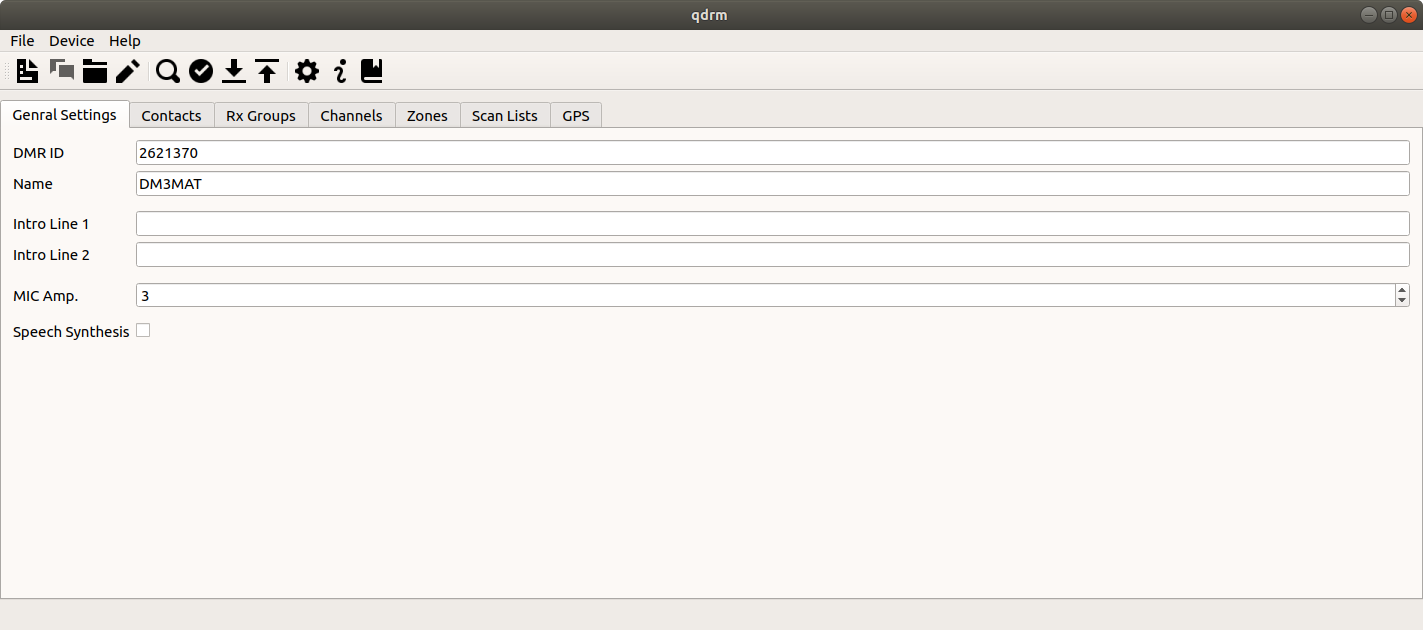
\includegraphics[width=0.75\linewidth]{../fig/qdmr-general-settings.png}
\end{center}
QDMR ist ein Versuch eine \emph{universelle} CPS zu bauen für verschiedene Geräte und Hersteller mit einem lesbaren code-plug und einer halbwegs modernen Oberfläche.
\end{frame}

\begin{frame}
 Unterstütze Geräte (bisher):
 \begin{itemize}
  \item Open GD-77 Firmware (RD-5R, GD-77, ...)
  \item Radioddity RD-5R
  \item Retevis RT3S
  \item TyT MD-UV390
  \item AnyTone AT-D878UV
 \end{itemize}
 \pause Quasi fertig:
 \begin{itemize}
  \item Radioddity GD-77
  \item TYT MD-UV380, MD-2017, MD-9600
  \item Retevis RT84
  \item Anytone AT-D868UVE
  \item BTECH DMR-6X2 (läuft wahrscheinlich schon, identisch zum AT-D878UV)
 \end{itemize}  
 \pause Nahe Zukunft:
 \begin{itemize}
  \item Hytera Geräte (vielen Dank an Matt)!
 \end{itemize}
\end{frame}

\begin{frame}
 \begin{center}
  {\Huge Demo!}
 \end{center}
\end{frame}

\begin{frame} \frametitle{Grundeinstellungen (1/5)}
\begin{center}
 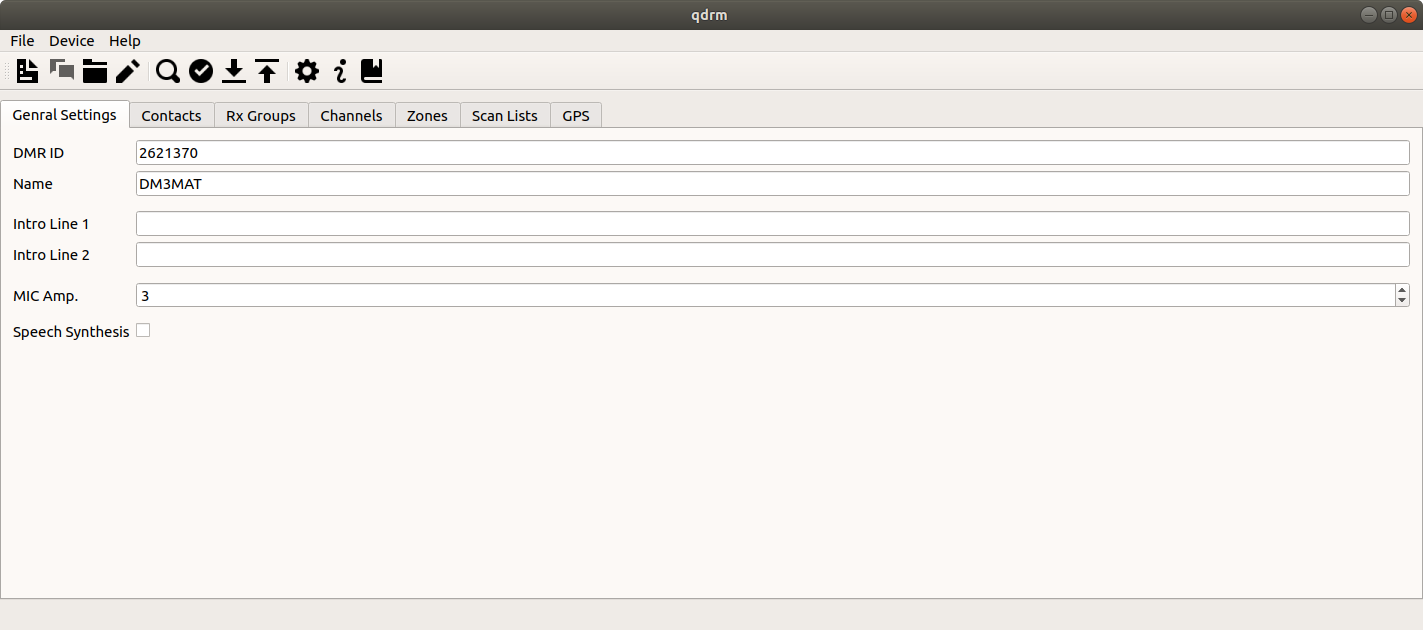
\includegraphics[width=0.75\linewidth]{../fig/qdmr-general-settings.png}
\end{center}
\end{frame}

\begin{frame} \frametitle{Kontakte/Sprechgruppen (2/5)}
\begin{center}
 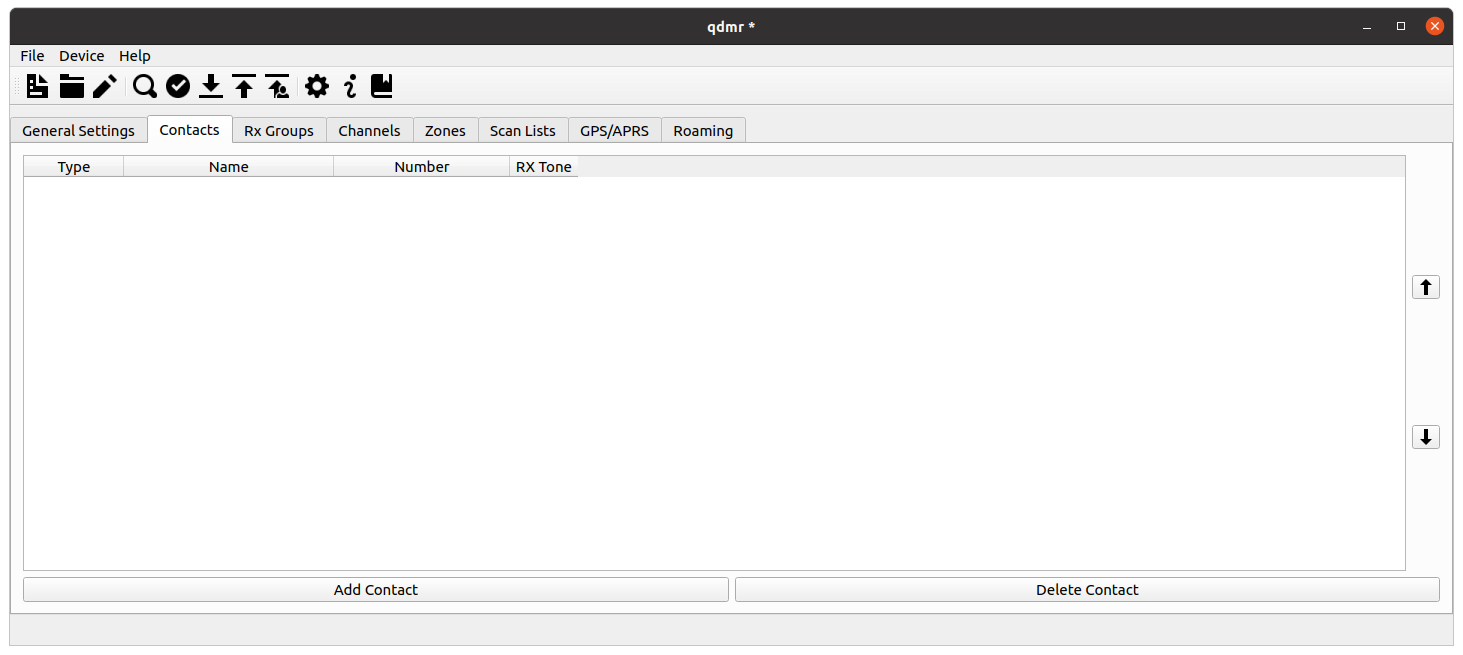
\includegraphics[width=0.75\linewidth]{../fig/qdmr-contacts-empty.png}
\end{center}
\end{frame}

\begin{frame} \frametitle{Kontakte/Sprechgruppen: Direktruf}
\begin{center}
 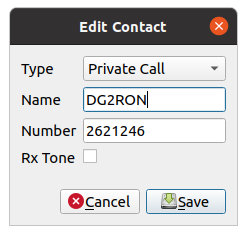
\includegraphics[width=0.25\linewidth]{../fig/qdmr-edit-contact-private-call.png}
\end{center}
\end{frame}

\begin{frame} \frametitle{Kontakte/Sprechgruppen: Gruppenruf}
\begin{center}
 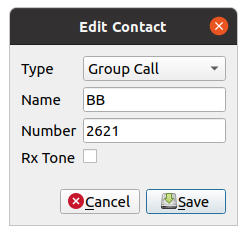
\includegraphics[width=0.25\linewidth]{../fig/qdmr-edit-contact-group-call.png}
\end{center}
\end{frame}

\begin{frame} \frametitle{Kontakte/Sprechgruppen (2/5)}
\begin{center}
 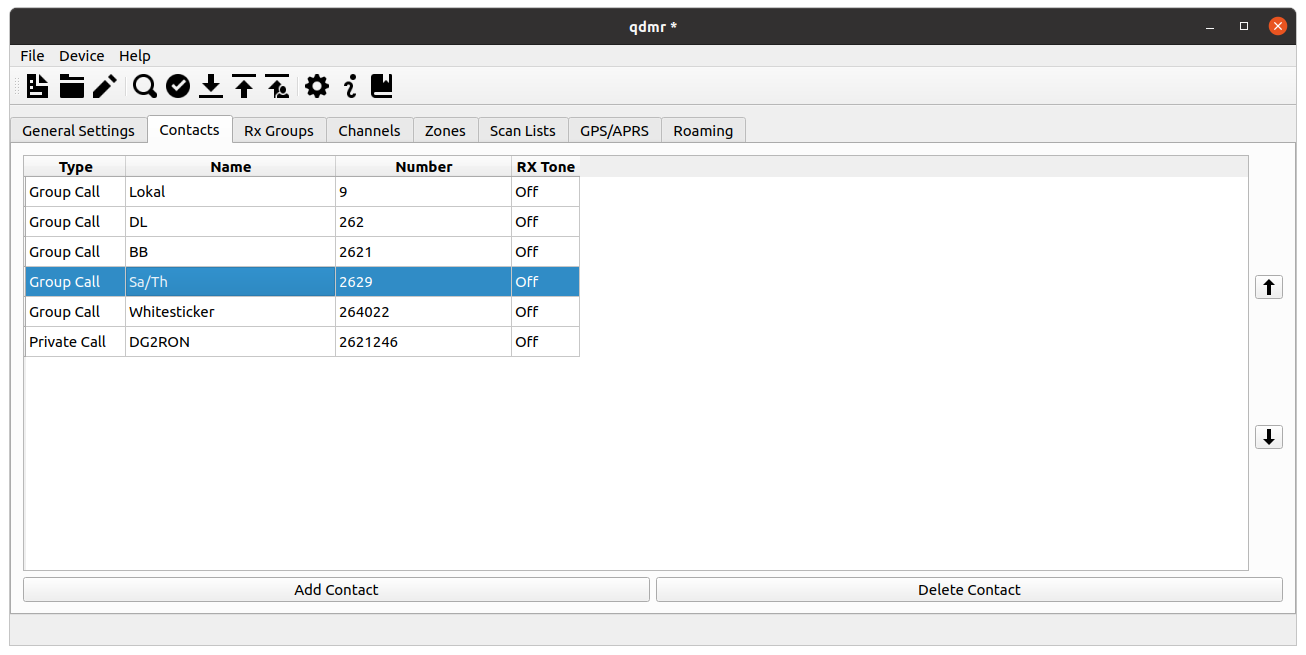
\includegraphics[width=0.75\linewidth]{../fig/qdmr-contacts-example.png}
\end{center}
\end{frame}

\begin{frame} \frametitle{Empfangsgruppen (3/5)}
\begin{center}
 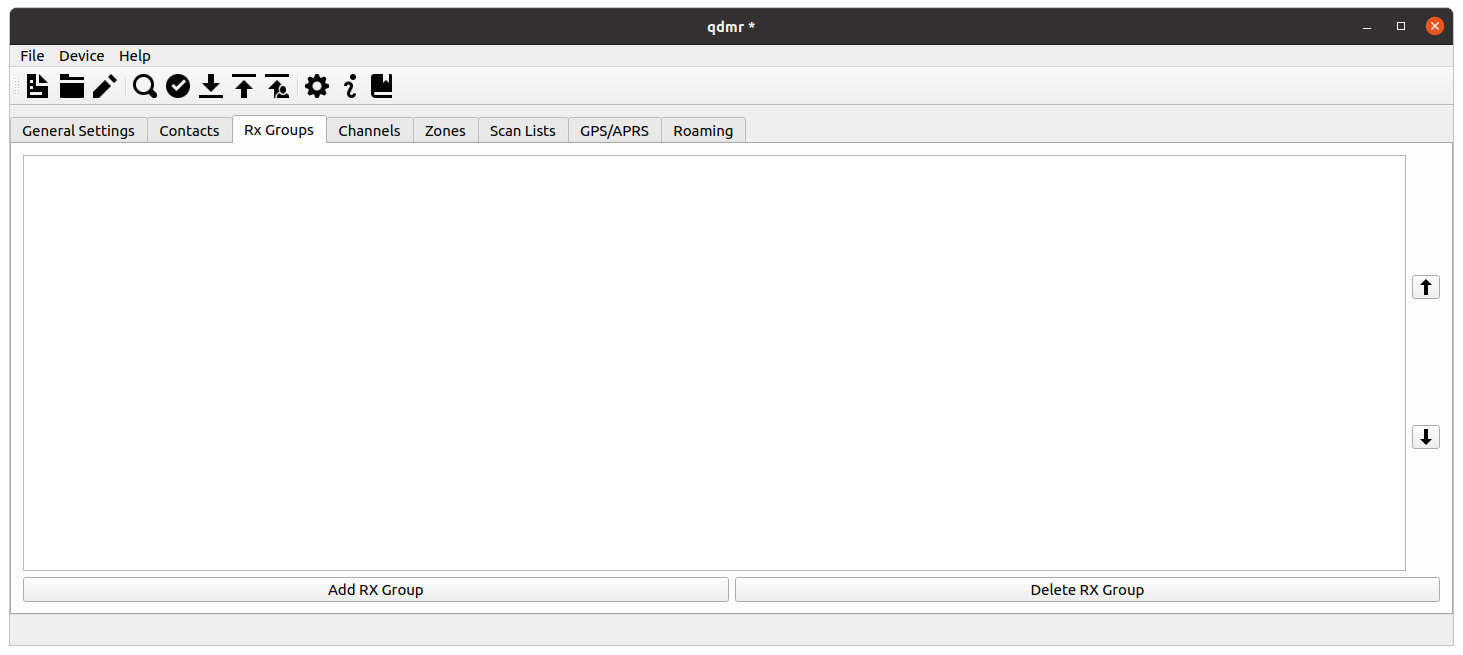
\includegraphics[width=0.75\linewidth]{../fig/qdmr-rxgroup-empty.png}
\end{center}
\end{frame}

\begin{frame} \frametitle{Empfangsgruppen: Hinzufügen}
\begin{center}
 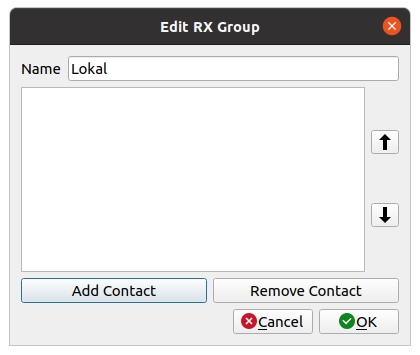
\includegraphics[width=0.25\linewidth]{../fig/qdmr-edit-rxgroup-empty.png}
\end{center}
\end{frame}

\begin{frame} \frametitle{Empfangsgruppen: Hinzufügen}
\begin{center}
 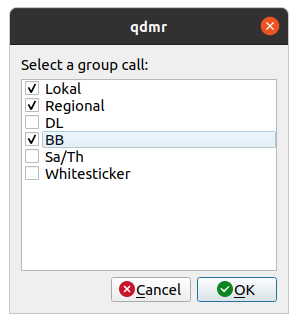
\includegraphics[width=0.25\linewidth]{../fig/qdmr-edit-rxgroup-select.png}
\end{center}
\end{frame}

\begin{frame} \frametitle{Empfangsgruppen (3/5)}
\begin{center}
 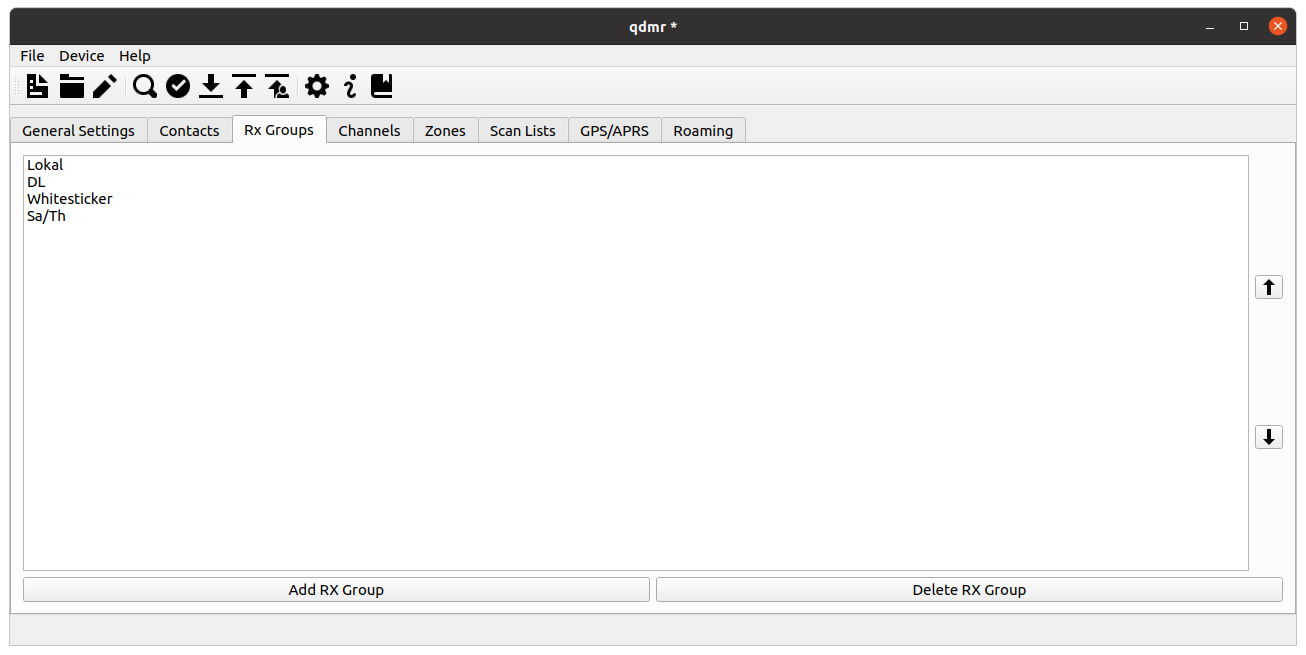
\includegraphics[width=0.75\linewidth]{../fig/qdmr-rxgroup-list.png}
\end{center}
\end{frame}

\begin{frame} \frametitle{Kanäle (4/5)}
\begin{center}
 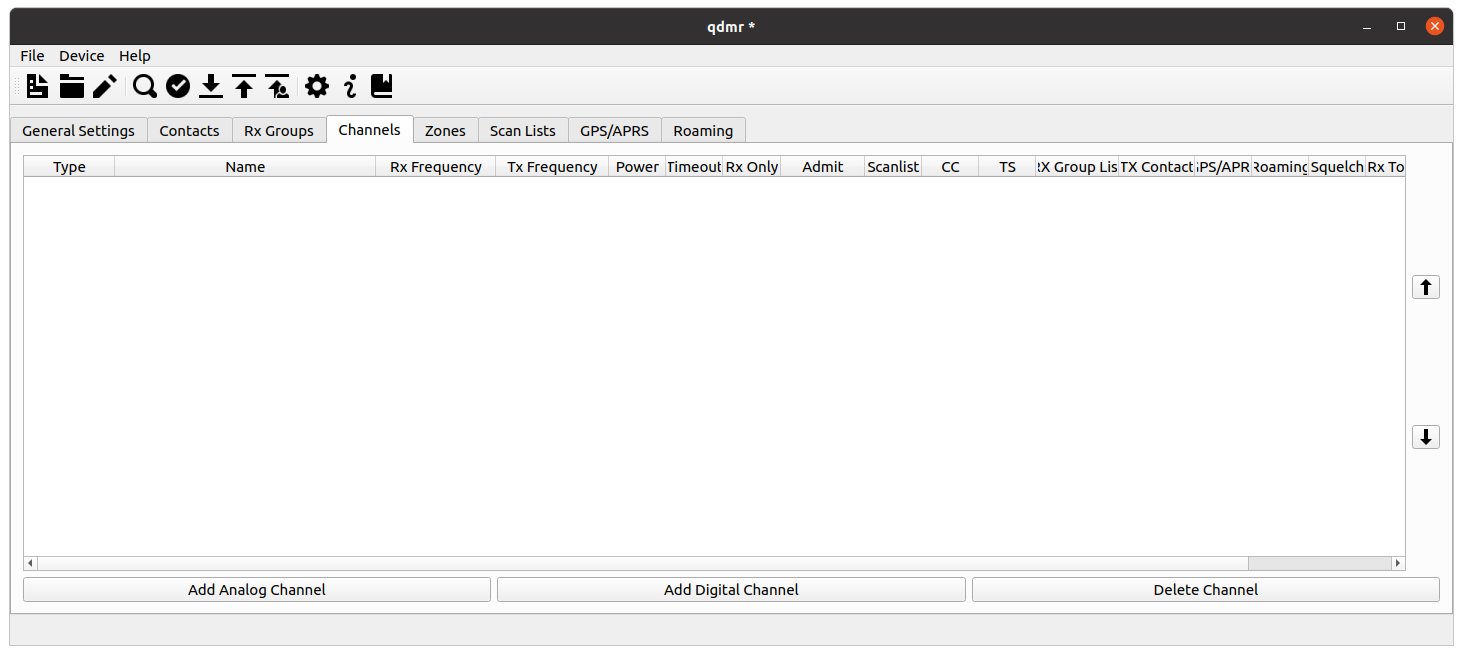
\includegraphics[width=0.75\linewidth]{../fig/qdmr-channels-empty.png}
\end{center}
\end{frame}

\begin{frame} \frametitle{Kanäle: Analog}
\begin{center}
 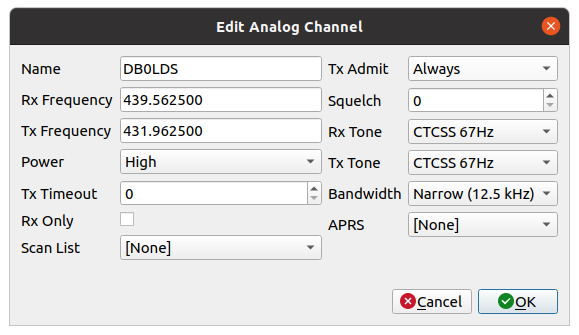
\includegraphics[width=0.5\linewidth]{../fig/qdmr-channels-edit-analog.png}
\end{center}
\end{frame}

\begin{frame} \frametitle{Kanäle: Digital}
\begin{center}
 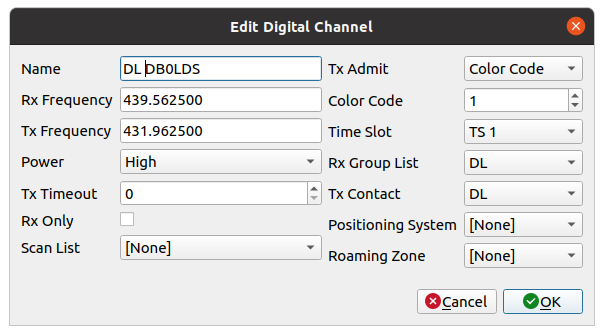
\includegraphics[width=0.5\linewidth]{../fig/qdmr-channels-edit-digital.png}
\end{center}
\end{frame}

\begin{frame} \frametitle{Kanäle (4/5)}
\begin{center}
 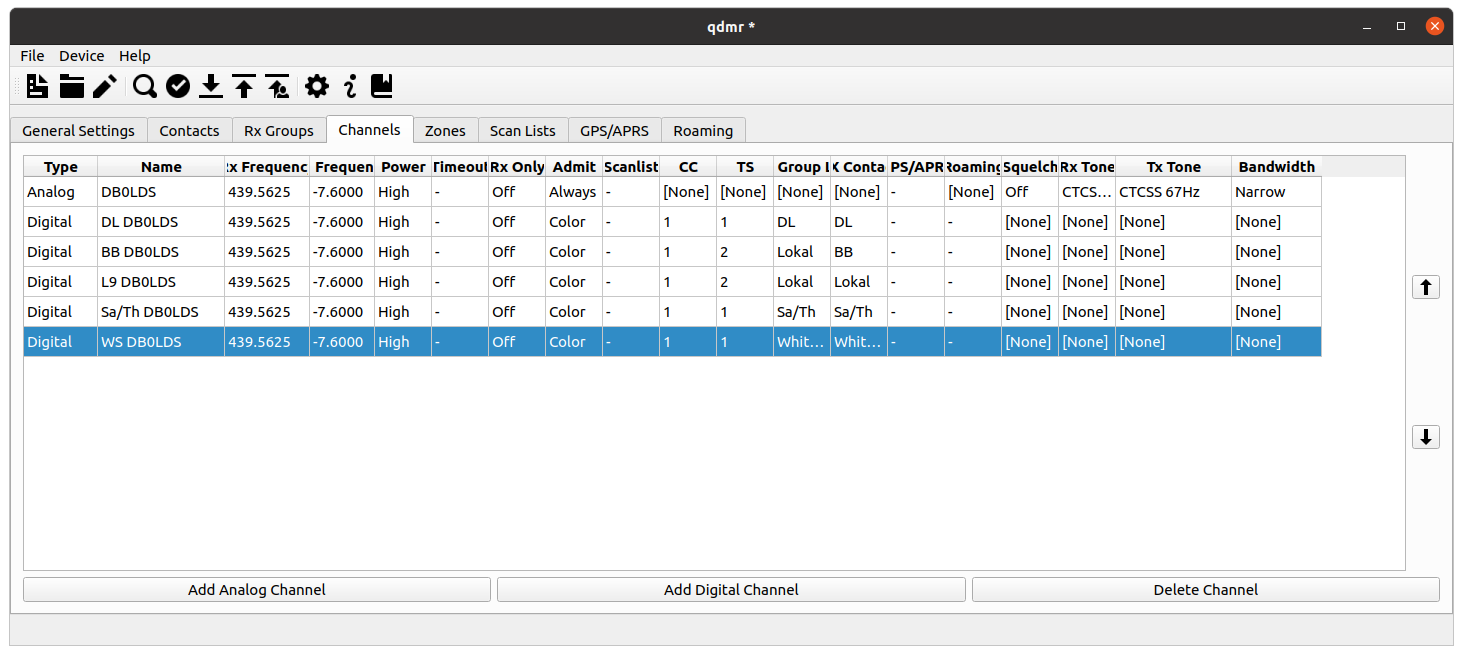
\includegraphics[width=0.75\linewidth]{../fig/qdmr-channels-example.png}
\end{center}
\end{frame}

\begin{frame} \frametitle{Zonen (5/5)}
\begin{center}
 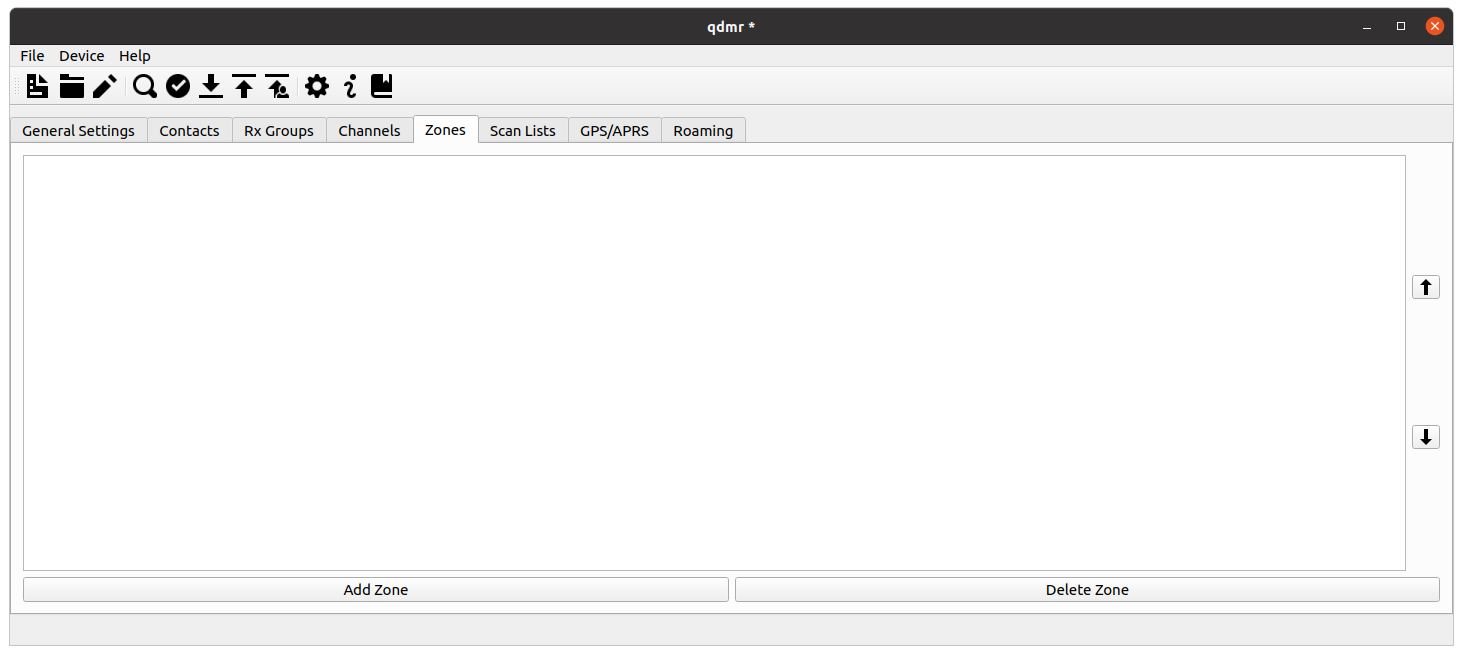
\includegraphics[width=0.75\linewidth]{../fig/qdmr-zone-empty.png}
\end{center}
\end{frame}

\begin{frame} \frametitle{Zone hinzufügen}
\begin{center}
 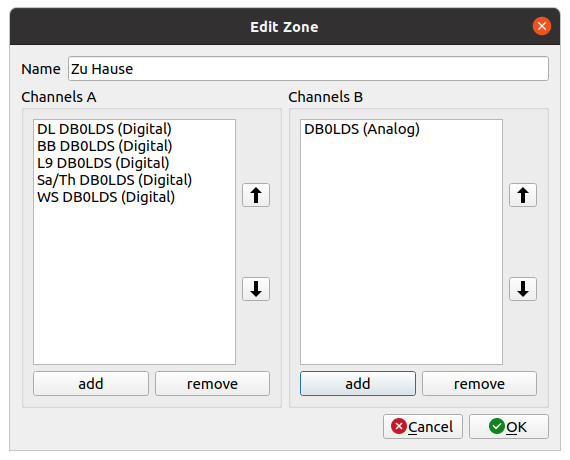
\includegraphics[width=0.5\linewidth]{../fig/qdmr-zone-edit.png}
\end{center}
\end{frame}

\begin{frame} \frametitle{Kanäle zur Zone hinzufügen}
\begin{center}
 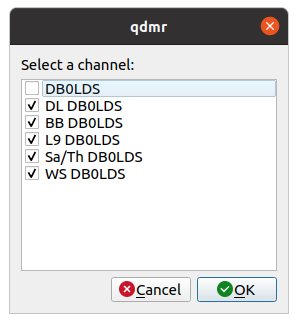
\includegraphics[width=0.25\linewidth]{../fig/qdmr-zone-edit-select.png}
\end{center}
\end{frame}

\begin{frame} \frametitle{Zonen (5/5)}
\begin{center}
 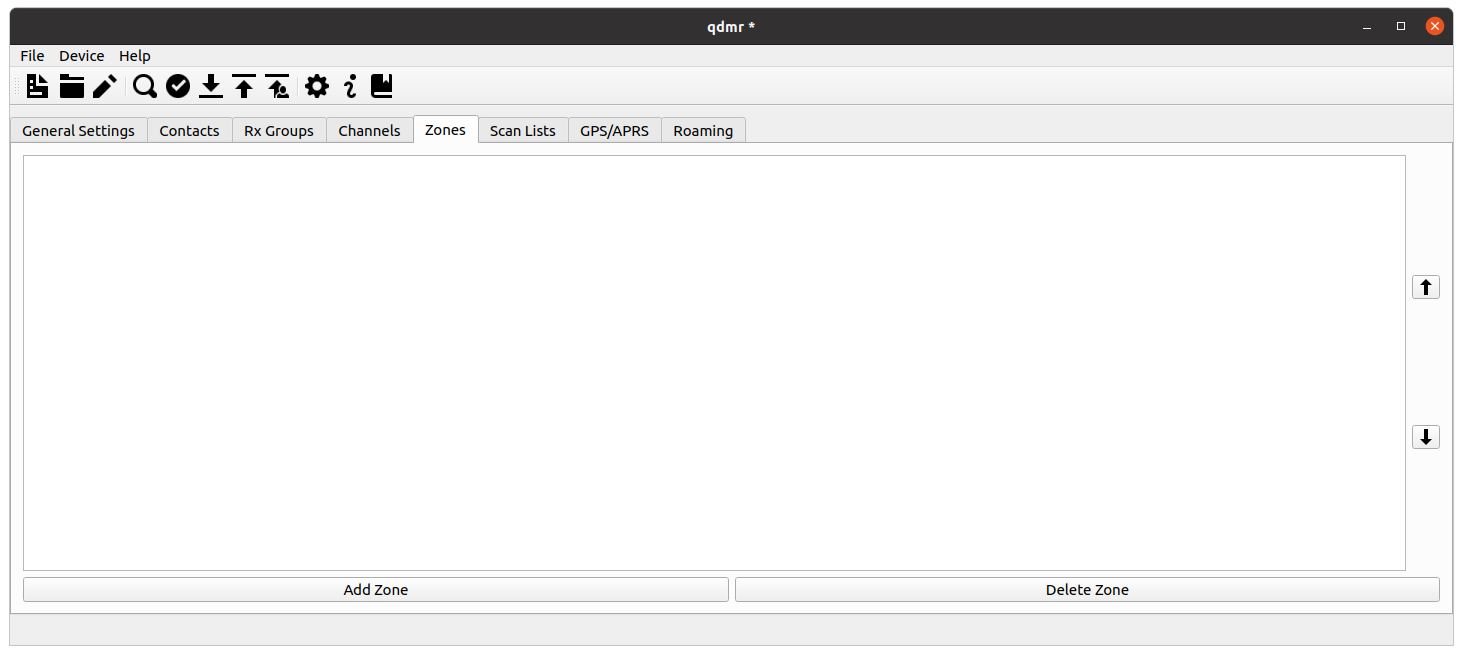
\includegraphics[width=0.75\linewidth]{../fig/qdmr-zone-empty.png}
\end{center}
\end{frame}

\begin{frame} \frametitle{Code-plug Format}
\begin{center}
 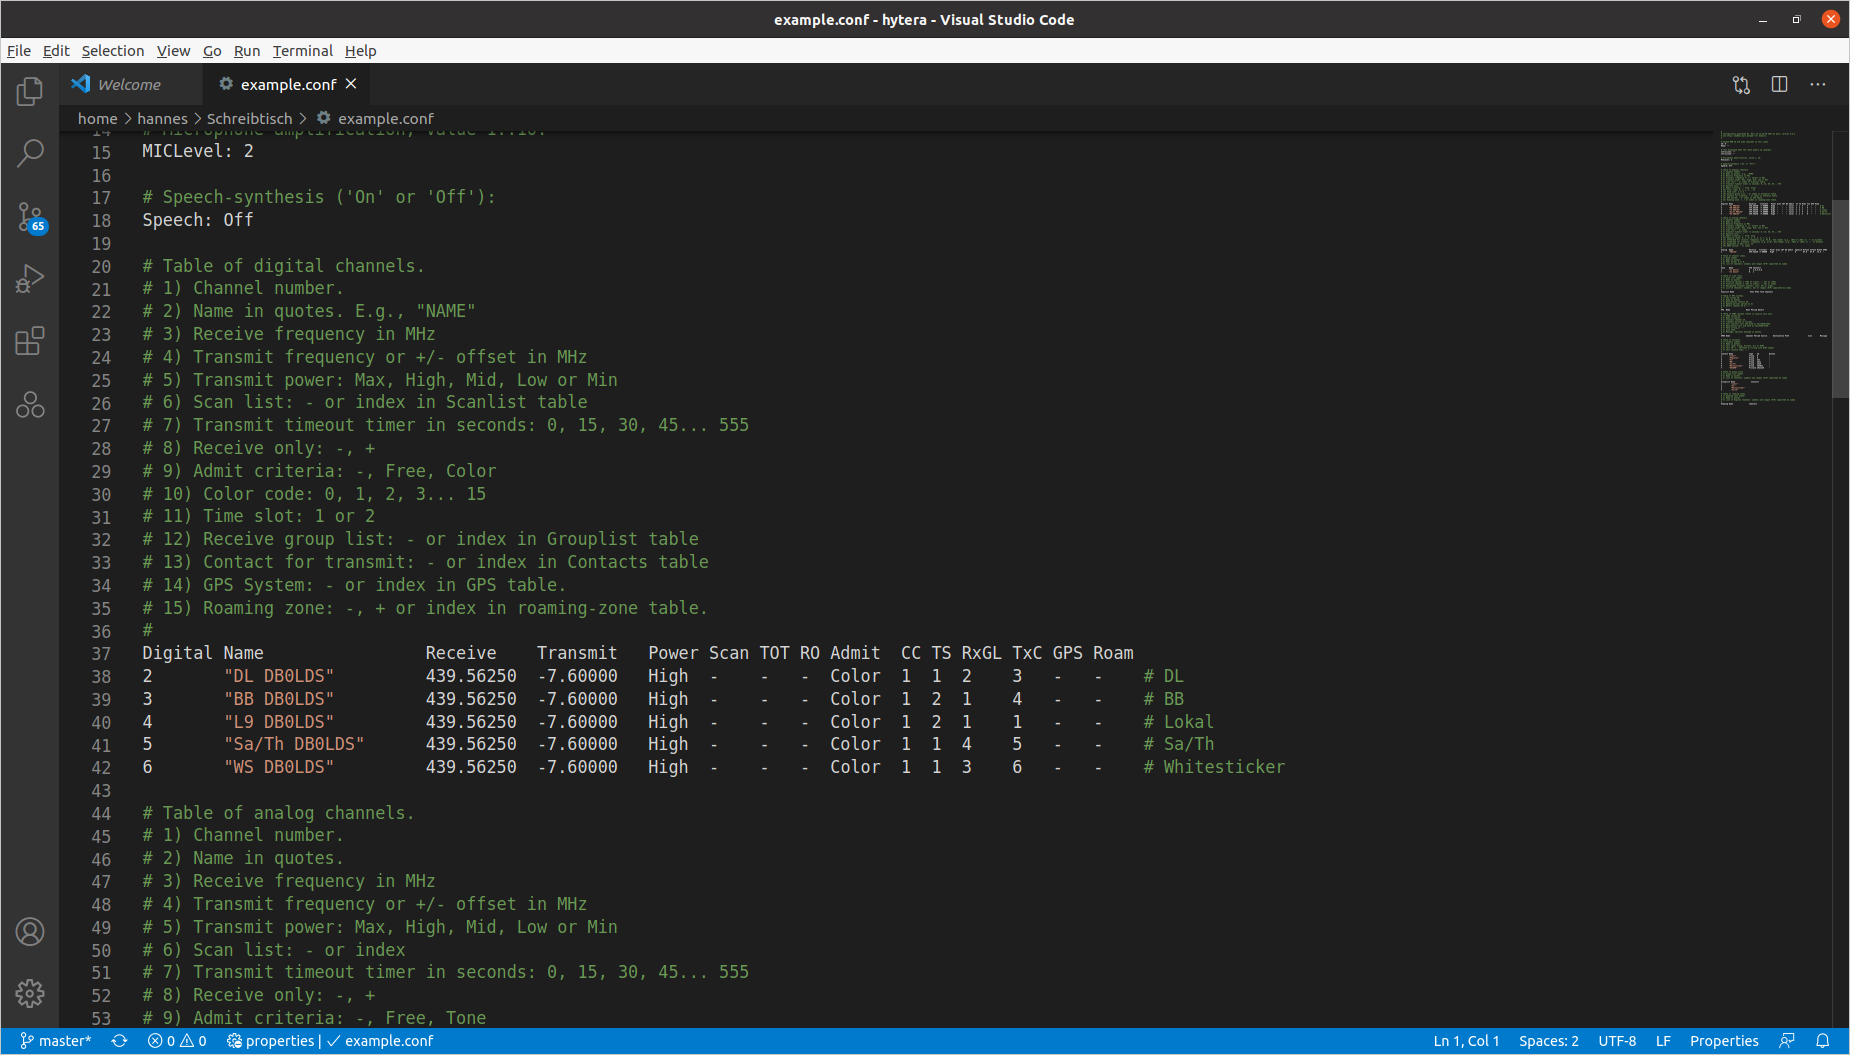
\includegraphics[width=0.9\linewidth]{../fig/qdmr-codeplug-format.png}
\end{center}
\end{frame}


\section{Down the rabbit hole}
\begin{frame} \frametitle{Howto reverse engineer a code-plug?}
 Hilfsmittel:
 \begin{itemize}
  \item Eine Windows Instanz in einer virtuellen Maschine (VirtualBox, o.ä.) mit der original CPS
  \item Wireshark mit \emph{usbmon} Kernelmodul (bei allen Linux Distributionen dabei)
  \item Viel Geduld
  \item Viel Frustrationstoleranz
 \end{itemize}
 Vorgehen:
 \begin{itemize}
  \item Die Kommunikation zwischen CPS und Gerät belauschen und mitschneiden.
  \item Die Rohdaten aus den Mitschnitten extrahieren und Gemeinsamkeiten/Unterschiede darin finden.
  \item Daraus das Kommunikationsprotokoll sowie das Paketformat ableiten (sehr aufwendig).
  \item Danach differentielle Analyse des Code-plugs. D.h., 
  \begin{itemize}
    \item \textbf{Eine} kleine Änderung im code-plug auf das Gerät spielen.
    \item Kommunikation mitschneiden
    \item Code-plug daraus extrahieren.
    \item Vergleichen vor und nach der Änderung.
  \end{itemize}
 \end{itemize}
\end{frame}

\begin{frame}[fragile]\frametitle{Howto reverse engineer a code-plug?}
Beispiel Hytera (Rohdaten):
\begin{verbatim}
7e 00 00 fe 20 10 00 00 00 0c 60 e5
7e 01 00 00 20 10 00 00 00 14 31 d3 02 03 02 01 00 00 2c 03    
7e 01 00 00 20 10 00 00 00 24 02 f1 02 c5 01 11 00 [...] 00 5b 03
7e 01 00 00 20 10 00 00 00 14 41 c3 02 01 02 01 00 12 1c 03    
\end{verbatim}
\end{frame}

\begin{frame}[fragile]\frametitle{Howto reverse engineer a code-plug?}
Beispiel Hytera (Code-plug extrahieren):
\begin{lstlisting}
< RES: flags=00, src=10, dest=20, seq=0004
  | RSP: type=81C7 seq=EA crc=170F (1887)
  | RD: addr=00000000
  | |  00000000 16 01 52 43 44 42 01 db 07 02 18 50 44 37 38 30 | ..RCDB.....PD780
  | |  00000010 30 30 47 30 30 4d 30 30 30 30 30 00 00 85 85 00 | 00G00M00000.....
  | |  00000020 00 00 00 00 00 00 56 6a 19 00 9a 00 00 00 00 00 | ......Vj........
...
\end{lstlisting}
\end{frame}

\begin{frame}[fragile]\frametitle{Howto reverse engineer a code-plug?}
Beispiel Hytera (Code-plug vergleichen, einfach mit \emph{diff}):
Hier wurde gar nichts geändert, dennoch gibt es einen unterschied im übertragenen Code-plug
\begin{lstlisting}
< 00000090 80 a1 03 1c e5 07 03 16 02 17 db 07 03 0a 0a 21 | ...............!
---
> 00000090 80 a1 03 1c e5 07 03 16 02 1a db 07 03 0a 0a 21 | ...............!
\end{lstlisting}
\begin{itemize}
 \item \texttt{0x07e3} = 2021, \texttt{0x03} = 3, \texttt{0x16} = 22, \texttt{0x02} = 2, \texttt{0x17}=23
 \item \texttt{0x07e3} = 2021, \texttt{0x03} = 3, \texttt{0x16} = 22, \texttt{0x02} = 2, \texttt{0x1a}=26
 \item $\Rightarrow$ Unterschied ist Zeitstempel der letzten Programmierung.
\end{itemize}
\end{frame}

\begin{frame}[fragile]\frametitle{Howto reverse engineer a code-plug?}
Beispiel Hytera (Code-plug vergleichen, einfach mit \emph{diff}):
Hier wurde die DMR ID von 1 auf 12345678 geändert:
\begin{lstlisting}
< 00065AA0 04 00 4c 00 00 00 62 00 00 00 01 00 00 00 10 06 | ..L...b.........
---
> 00065AA0 04 00 4c 00 00 00 62 00 00 00 4e 61 bc 00 10 06 | ..L...b...Na....
\end{lstlisting}
\begin{itemize}
 \item \texttt{0x01} = 1, \texttt{0xbc614e} = 12345678
 \item $\Rightarrow$ Die DMR ID wird an der Adresse \texttt{0x00065AAA} als 24bit little-endian Zahl abgelegt.
\end{itemize}
\end{frame}

\end{document}